\chapter{Diseño e Implementación} % Main chapter title

\label{Chapter3} % Change X to a consecutive number; for referencing this chapter elsewhere, use \ref{ChapterX}
\definecolor{mygreen}{rgb}{0,0.6,0}
\definecolor{mygray}{rgb}{0.5,0.5,0.5}
\definecolor{mymauve}{rgb}{0.58,0,0.82}

\lstset{ %
  backgroundcolor=\color{white},   % choose the background color; you must add \usepackage{color} or \usepackage{xcolor}
  basicstyle=\footnotesize,        % the size of the fonts that are used for the code
  breakatwhitespace=false,         % sets if automatic breaks should only happen at whitespace
  breaklines=true,                 % sets automatic line breaking
  captionpos=b,                    % sets the caption-position to bottom
  commentstyle=\color{mygreen},    % comment style
  deletekeywords={...},            % if you want to delete keywords from the given language
  %escapeinside={\%*}{*)},          % if you want to add LaTeX within your code
  %extendedchars=true,              % lets you use non-ASCII characters; for 8-bits encodings only, does not work with UTF-8
  %frame=single,	                   % adds a frame around the code
  keepspaces=true,                 % keeps spaces in text, useful for keeping indentation of code (possibly needs columns=flexible)
  keywordstyle=\color{blue},       % keyword style
  language=[ANSI]C,					% the language of the code
  %otherkeywords={*,...},           % if you want to add more keywords to the set
  numbers=left,                    % where to put the line-numbers; possible values are (none, left, right)
  numbersep=5pt,                   % how far the line-numbers are from the code
  numberstyle=\tiny\color{mygray}, % the style that is used for the line-numbers
  rulecolor=\color{black},         % if not set, the frame-color may be changed on line-breaks within not-black text (e.g. comments (green here))
  showspaces=false,                % show spaces everywhere adding particular underscores; it overrides 'showstringspaces'
  showstringspaces=false,          % underline spaces within strings only
  showtabs=false,                  % show tabs within strings adding particular underscores
  stepnumber=1,                    % the step between two line-numbers. If it's 1, each line will be numbered
  stringstyle=\color{mymauve},     % string literal style
  tabsize=2,	                   % sets default tabsize to 2 spaces
  title=\lstname,                   % show the filename of files included with \lstinputlisting; also try caption instead of title
  morecomment=[s]{/*}{*/}%
}

En este capítulo se presenta como caso de estudio el funcionamiento del software de depuración para programas en C mediante Eclipse IDE y se describe en detalle el desarrollo del diseño e implementación del sistema para depuración elegido. 

%----------------------------------------------------------------------------------------
%	SECTION 1
%----------------------------------------------------------------------------------------

\section{Descripción general}
\label{sec:Descripción general}

El sistema se compone de una computadora ejecutando la depuración de un programa en lenguaje CIAABOT, y la placa EDU-CIAA-NXP conectado a la computadora, por medio de una interfaz, desde donde el IDE del \emph{debug} realice la comunicación con el hardware como se muestra en la figura \ref{fig:pc-bloques}.

\begin{figure}[!htbp]
    \begin{center}  % [width=10cm,height=5cm] [width=\textwidth]
	\includegraphics*[width=10cm,height=5cm]{./Figures/pc-bloques.png}
	\par\caption{Modelo conceptual.}\label{fig:pc-bloques}
	\end{center}
\end{figure}


\section{Caso de estudio: depuración con eclipse}
\label{sec:Alternativa de diseño}

Para diseñar el software de depuración se toma como caso de estudio la depuración de programas escritos en lenguaje C con Eclipse IDE sobre la EDU-CIAA-NXP:

\begin{itemize}
	\item \emph{Plugin de eclipse arm-none-eabi-gdb}
	\footnote{Software de configuración de eclipse para usar el depurador GNU para procesadores ARM Cortex-A/R/M.}: realiza la interpretación de comandos de	GDB-MI y muestra los resultados en la interfaz gráfica del editor de texto de C en el IDE del Eclipse.
	\item \emph{arm-none-eabi-gdb}: software de debug originario de Linux que realiza el mapeo de los símbolos de C con las instrucciones en código máquina que se ejecutan en el microcontrolador (mapea las funciones al código binario en flash), para
	luego permitir ejecutar los comandos de parar, continuar o de uso de brakpoints.
	\item \emph{OpenOCD (Open On-Chip Debugger)}: software de código abierto que interactúa con el puerto JTAG de un depurador de hardware, provee a GDB el remote interface protocol para permitirle acceder al hardware. Traduce transacciones JTAG o SWD (mediante el puerto serie sobre USB) a comandos remote-protocol de GDB. OpenOCD utiliza scripts de configuración (archivos *.cfg) donde se describe el microcontrolador a depurar y la interfaz de hardware para acceder al mismo (en adelante \emph{"Debugger HW"}).
	\item \emph{Debugger HW}: en el caso de la EDU-CIAA es el circuito de interfaz fisica para pasar de JTAG a USB (modo puerto serie virtual). En la EDU-CIAA
	viene incluido en la misma placa que se encuentra el microcontrolador a depurar.
	\item \emph{Microcontrolador a depurar}: El microcontrolador posee un periferico específico para \emph{debug} con interfaz JTAG (Acrónimo de Joint Test Action Group, es utilizado como mecanismo para depuración de sistemas embebidos, proveendo una puerta trasera para acceder al sistema) teniendo acceso para modificar la RAM, Flash y los registros del Microcontrolador.
\end{itemize}

Una alternativa para la programación de un software de depuración a nivel de bloques de CIAABOT es, entonces, mantener el mapeo entre los bloques de programa de CIAABOT y su C generado, y comunicarse con GDB, mediante GDB-MI como lo realiza el plugin de Eclipse.

Teniendo en cuenta la complejidad de implementar lo expuesto, se propone como una alternativa factible, el de emular la funcionalidad de \emph{debugger} mediante la ejecución del programa de CIAABOT en la propia PC, de manera que al momento de ejecutarse los bloques gráficos de acceso a los periféricos, se realice la comunicación con la placa mediante un protocolo, para realizar la ejecución de comandos de lectura y escritura en los periféricos que se requiera manipular.

Como protocolo de comunicación para acceso al hardware se elije utilizar el protocolo firmata, debido a que existe una implementación del mismo para la EDU-CIAA-NXP \citep{CIAA:firmwarev2} y existen múltiples bibliotecas firmata para diferentes lenguajes de programación en la PC.  

\subsection{Firmata}
\label{subsec:Firmata}

Firmata es un protocolo genérico y abierto, fue diseñado para la comunicación directa entre un microcontrolador previamente instalado con un programa que implementa firmata y un objeto de software que implementa un cliente firmata en una computadora host. 

El protocolo se puede implementar en cualquier arquitectura de microcontroladores, así como en cualquier paquete de software.

Firmata4CIAA es un programa que implementa el protocolo firmata en la EDU-CIAA-NXP. En la figura \ref{fig:componentesFirmata} se muestra el uso de firmata con la EDU-CIAA-NXP.

\begin{figure}[h]
	\centering
	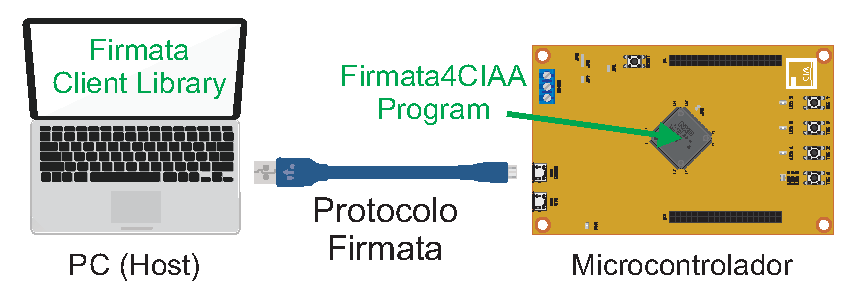
\includegraphics[scale=.80]{./Figures/Firmata4CIAA_01.pdf}
	\caption{Uso de firmata con la Educiaa.}
	\label{fig:componentesFirmata}
\end{figure}

\section{Sistema para depuración propuesto}
\label{section:Sistema para depuración propuesto}

El funcionamiento del entorno propuesto se puede resumir en los siguientes pasos:

\begin{itemize}
	\item Ejecutar un programa bloque a bloque en la PC, usando Javascript internamente, hasta que se encuentre con un bloque que requiera acceso a algún periférico del hardware.
	\item Enviar comandos firmata a la placa cuando se encuentre un bloque de acceso a algún periférico.
	\item Visualizar el contenido de las variables en un determinado momento de la ejecución.
	\item Instalación del programa que implementa el protocolo firmata en la EDU-CIAA-NXP, sólo en el caso de ser necesario.
\end{itemize}	

Cabe destacar que los bloques gráficos que acceden a los periféricos,
serán más lentos que si se tuviera que implementar mediante GDB-MI, ya que ese programa accedería al hardware a la velocidad en la que
se llama a las instrucciones del hardware, debido al código binario compilado
instalado en la placa.

Por el contrario, los bloques gráficos que no acceden a los periféricos, en tiempo
de ejecución, serán más rápidos, debido a que se ejecutarán directamente en la
misma PC del usuario. El programa se ejecutará dentro del contexto de la máquina virtual de
JavaScript, que es más rápido que el código C compilado en el microcontrolador.

De esta manera si se miden los tiempos de ensayos, cuando se instala el firmware
del código C generado en la placa contra la ejecución de los bloques con firmata, estos tiempos no serán los mismos.

Una ventaja para el usuario de CIAABOT, es que podrá depurar el programa sin necesidad de esperar el tiempo de compilación del código C generado a partir del programa en bloques (especialmente en Windows) y descarga a la plataforma reduciendo los tiempos de desarrollo del programa.


\section{Características del entorno \emph{CIAABOT Debug}}
\label{sec:Características del entorno CIAABOT debug}

El Entorno de Programación de \emph{CIAABOT Debug} debe ser capaz de permitirle al usuario realizar las siguientes tareas:

\begin{itemize}
	\item Abrir o importar un programa realizado en CIAABOT IDE.
	\item Ejecutar un programa bloque a bloque.	
	\item Establecer puntos de interrupción  (puntos de parada en los bloques).
	\item Permitir la visualización del valor de las variables durante la ejecución del programa.
	\item Ejecución del programa con o sin puntos de interrupciones activos (\emph{breakpoints}).
	\item Pausar y parar la ejecución del programa desde cualquier momento dado.
	\item Descarga del programa que implementa el protocolo firmata en la EDU-CIAA-NXP, sólo en el caso de ser necesario.
\end{itemize}

Los proyectos creados en CIAABOT IDE son guardados como archivos con extensión .cbp, la misma contiene la información del proyecto, su nombre, el modelo de CIAABOT utilizado
y el diagrama en bloques. Un proyecto puede abrirse desde el entorno de \emph{debug}, la información del proyecto es cargada y el diagrama en bloques es mostrado.

\section{Interfaz gráfica de \emph{CIAABOT Debug}}
La figura \ref{fig:debug-modos} expone el diseño realizado para la interfaz gráfica de \emph{CIAABOT Debug}.


\begin{figure}[!htbp]
	\begin{center}  % [width=10cm,height=5cm] [width=\textwidth]
		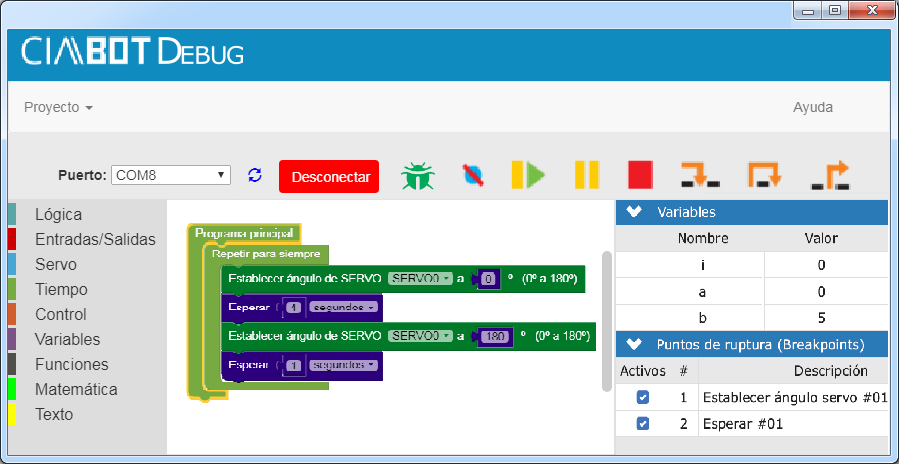
\includegraphics[width=15cm]{./Figures/CIAABOT-DEBUG-GUI-2.png}
		\par\caption{Diseño de la intergaz gráfica de \emph{CIAABOT Debug}.}\label{fig:debug-modos}
	\end{center}
\end{figure}


\emph{CIAABOT Debug} se compone de las siguientes partes:

\begin{itemize}
\item
Conexión con la plataforma.
\item
Editor de programa.	
\item
Iniciar sesión de depuración.
\item
Herramientas de control de ejecución.
\item
Menú de visualización de variables y puntos de interrupción.
\end{itemize}

En la figura \ref{fig:debug-modos} se resaltan cada una de ellas:

\begin{figure}[!htbp]
	\begin{center}  % [width=10cm,height=5cm] [width=\textwidth]
		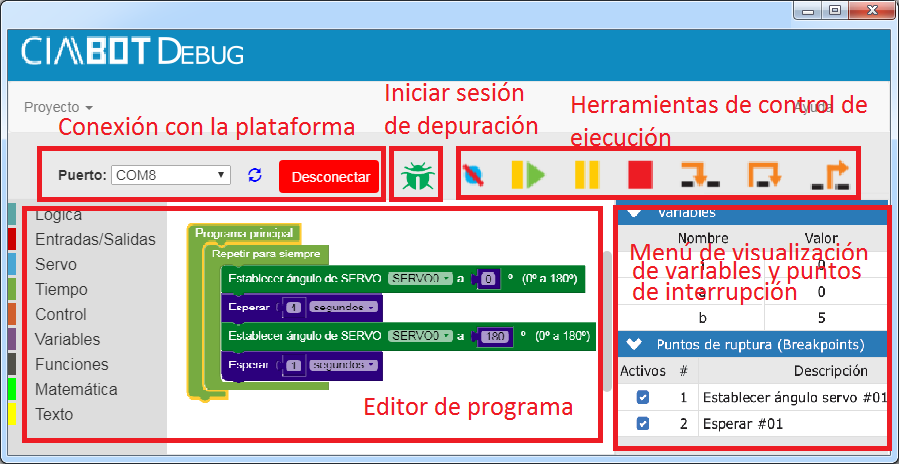
\includegraphics[width=15cm]{./Figures/CIAABOT-DEBUG-GUI-3.png}
		\par\caption{Composición de la intergaz gráfica de \emph{CIAABOT Debug}.}\label{fig:debug-modos}
	\end{center}
\end{figure}


\section{Máquina de estados de \emph{CIAABOT Debug}}
\label{sec:Modos de funcionamiento}

En la figura \ref{fig:diagrama-estados} se expone el diagrama de estados del software \emph{CIAABOT Debug}.


\begin{figure}[!htbp]
	\begin{center}  % [width=10cm,height=5cm] [width=\textwidth]
		\includegraphics*[width=15cm]{./Figures/diagrama-estados.pdf}
		\par\caption{Diagrama de máquina de estados de los modos de funcionamiento.}\label{fig:diagrama-estados}
	\end{center}
\end{figure}


\subsection{Desconectado}
\label{subsec:No Conectado}

La aplicación inicia en estado \emph{Desconectado}. En este modo de funcionamiento se permite la edición de bloques de programa, el botón de inicio de sesión de depuración se encuentra deshabilitado, así como las herramientas de control de ejecución. Mientras no este depurando se habilita la edición del programa. La figura \ref{fig:desconectado} expone la interfaz gráfica en este estado.


\begin{figure}[!htbp]
	\begin{center}  % [width=10cm,height=5cm] [width=\textwidth]
		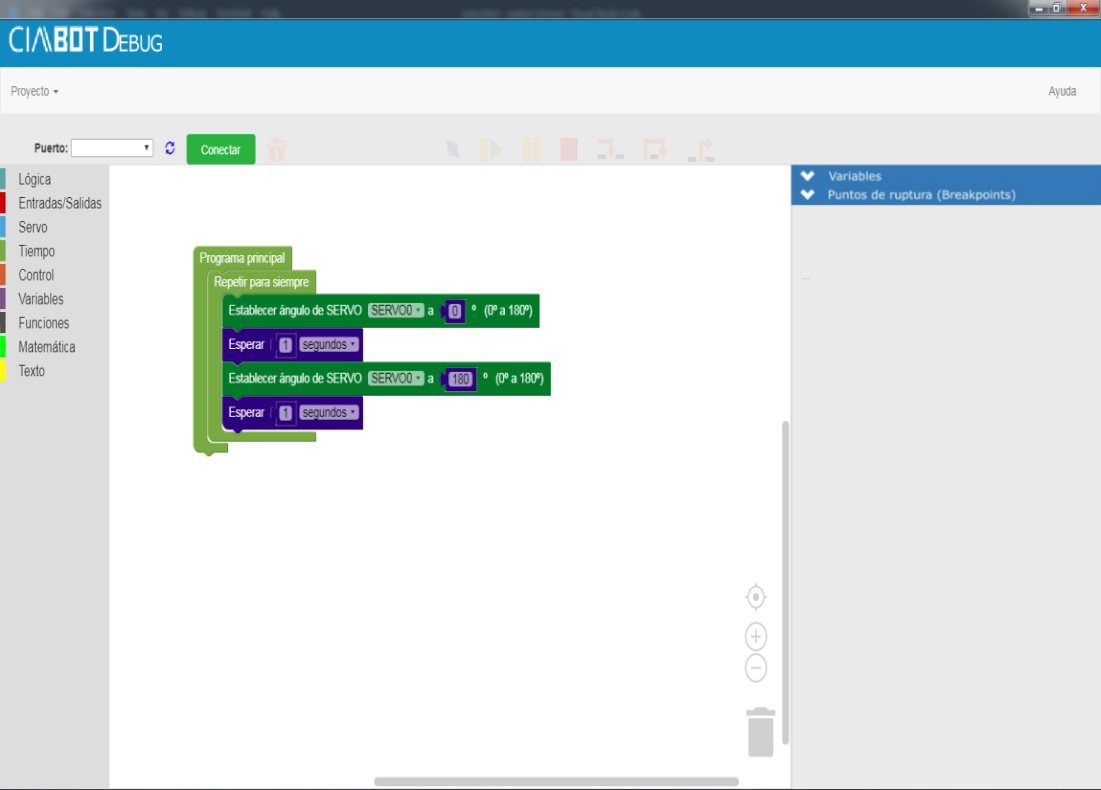
\includegraphics[width=15cm]{./Figures/debug-inicio.png}
		\par\caption{Estado Desconectado.}\label{fig:desconectado}
	\end{center}
\end{figure}


\subsection{Conectando}
\label{subsec:Conectando}

Cuando se presiona el botón “\emph{Conectar}” pasa al estado \emph{Conectando}. En este estado se permite la edición de bloques de programa y verifica si la EDU-CIAA-NXP tiene descargado el programa Firmata4CIAA, si lo tiene pasa a estado \emph{Conectado Con Firmata4CIAA}, sino pasa a \emph{Conectado Sin Firmata4CIAA}.

\subsection{Conectado Sin Firmata4CIAA}
\label{subsec:Conectado Sin Firmata4CIAA}

Si la aplicación paso a estado \emph{Conectado Sin Firmata4CIAA}, realiza la consulta al usuario si quiere descargar el programa Firmata4CIAA, si el usuario elige que sí, entonces se procede a realizar la descarga, y si elige que no entonces la aplicación vuelve al estado \emph{Desconectado}.

En la figura \ref{fig:instalar-firmata} muestra la consulta enviada al usuario.

\begin{figure}[!htbp]
	\begin{center}  % [width=10cm,height=5cm] [width=\textwidth]
		\includegraphics*[width=15cm]{./Figures/instalar-firmata.png}
		\par\caption{Descargar Firmata4CIAA.}\label{fig:instalar-firmata}
	\end{center}
\end{figure}

\subsection{Descargando Firmata4CIAA}
\label{subsec:Descargando Firmata4CIAA}

Firmata4CIAA, la aplicación pasa al estado \emph{Descargando Firmata4CIAA}. Si en medio del proceso existiese algún problema de descarga, se informará al usuario y volverá a estado \emph{Desconectado}.

Entre los archivos de \emph{CIAABOT Debug} se encuentra el proyecto de Firmata4CIAA previamente compilado para la EDU-CIAA-NXP. Para descargarlo el entorno requiere configurar la ruta del \emph{toolchain} y de \emph{OpenOCD}. Con esa información simplemente ejecuta el comando \emph{make download} en la ruta de dicho proyecto.

La figura \ref{fig:Configuracion} muestra la ventana desde donde se puede realizar la configuración de paths.

\begin{figure}[!htbp]
	\begin{center}  % [width=10cm,height=5cm] [width=\textwidth]
		\includegraphics*[width=12cm]{./Figures/Configuracion.PNG}
		\par\caption{Configuración de paths.}\label{fig:Configuracion}
	\end{center}
\end{figure}


\subsection{Conectado Con Firmata4CIAA}
\label{subsec:Conectado Con Firmata4CIAA}

En caso de que la conexión resulte exitosa y se compruebe la disponibilidad de Firmata en la plataforma, la aplicación pasa al estado \emph{Conectado Con Firmata4CIAA}, se habilita el inicio de sesión de depuración
En la figura \ref{fig:conectado} se muestra este modo de funcionamiento.


\begin{figure}[!htbp]
	\begin{center}  % [width=10cm,height=5cm] [width=\textwidth]
		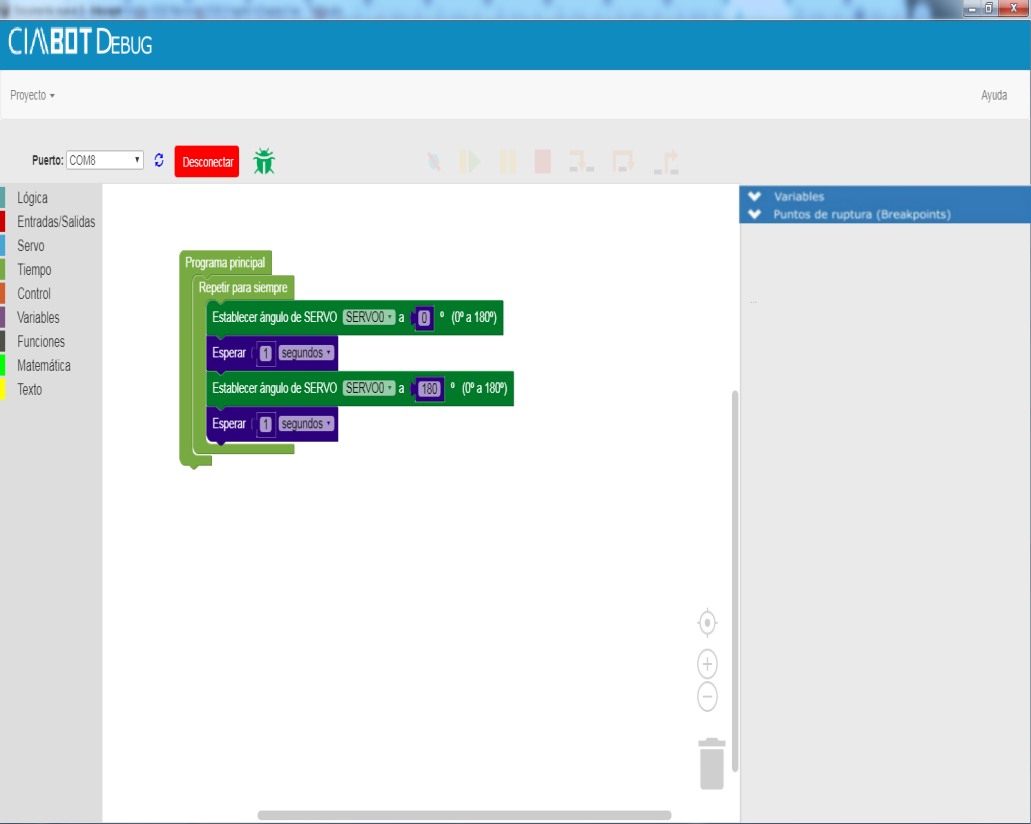
\includegraphics[width=15cm]{./Figures/debug-conectado.png}
		\par\caption{Estado Conectado con Firmata4CIAA.}\label{fig:conectado}
	\end{center}
\end{figure}

\subsection{Conectado En Sesión De Depuración}
\label{subsec:Conectado En Sesion De Depuración}

Si en el estado Conectado el usuario inicia la sesión de depuración, el entorno pasa a estado \emph{Conectado En Sesión de Depuración}. En este estado habilita la barra de herramientas de control de ejecución, permitiendole realizar el ensayo de su programa y deshabilita el menú de edición. La figura \ref{fig:debug} muestra la aplicación con este estado.

\begin{figure}[!htbp]
	\begin{center}  % [width=10cm,height=5cm] [width=\textwidth]
		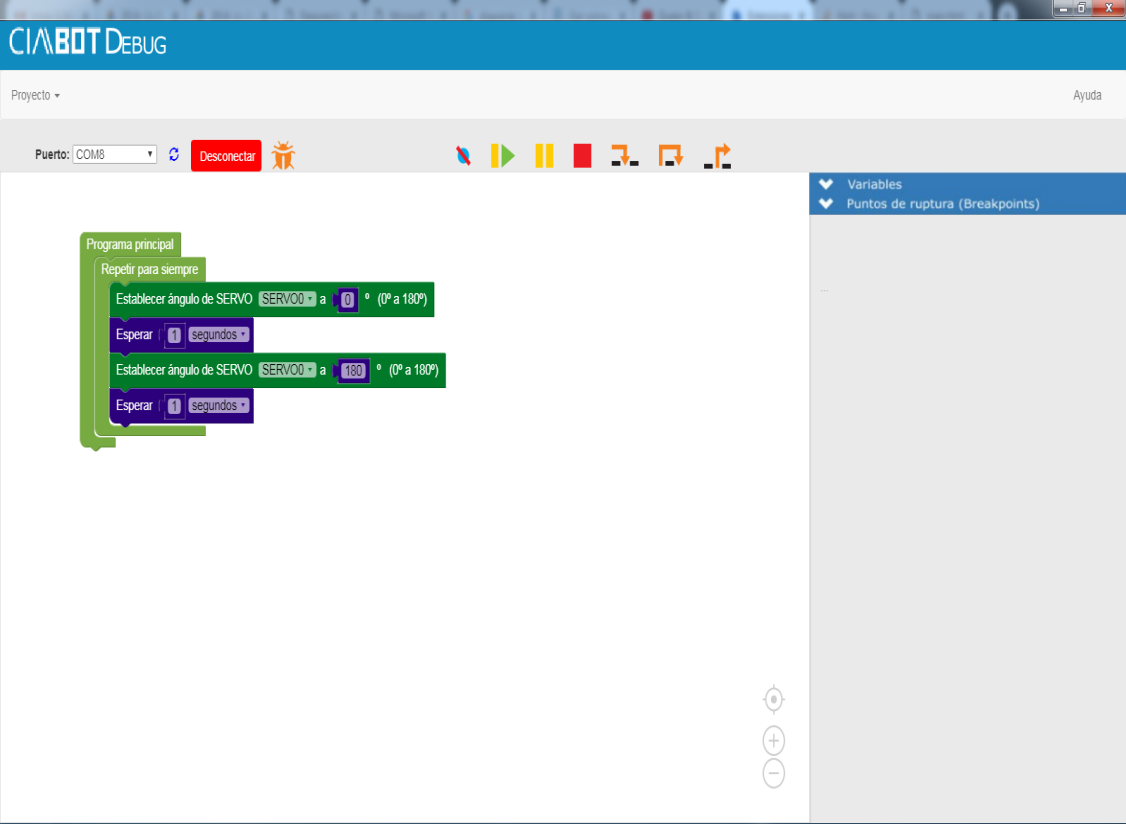
\includegraphics[width=15cm]{./Figures/debug-debug.png}
		\par\caption{Estado Depurando.}\label{fig:debug}
	\end{center}
\end{figure}


\section{Sesión de depuración}
\label{sec:Sesión de depuración}

\subsection{Iniciar/detener sesión}
\label{subsec:Iniciar/detener sesión}

Cuando inicia la aplicación el icono de \emph{debug} se muestra deshabilitado (color gris), como se muestra en la figura \ref{fig:debug_view_habilitada}.
Al tener la EDU-CIAA-NXP con Firmata4CIAA, la aplicación estará lista para iniciar la sesión de depuración, cambiando el icono de \emph{debug} de color gris (deshabilitado) a color verde (habilitado), de esta manera se permite al usuario mediante un click en el mismo, comenzar con la sesión de depuración. Al presionarlo, el botón se pone en color naranja, indicando que se ha iniciado una sesión de depuración y se deshabilita la acción de click sobre el mismo. Con la sesión de depuración iniciada el entorno habilita las herramientas de control de ejecución como se muestra en la figura \ref{fig:herramientas-control-ejecucion}.

\begin{figure}[h]
	\centering
	
\includegraphics[width=8cm]{./Figures/estadosBotonDebug.PNG}
	\caption{Estados del botón de depuración.}
	\label{fig:debug_view_habilitada}
\end{figure}


\begin{figure}[h]
	\centering
	
\includegraphics[width=10cm]{./Figures/herramientas-control-ejecucion.PNG}
	\caption{Herramientas de control de ejecución habilitada.}
	\label{fig:herramientas-control-ejecucion}
\end{figure}

La sesión de depuración finaliza cuando el usuario presiona el botón \emph{Detener depuración}, o si se cierra el programa en la aplicación.

\subsection{Herramientas de control de ejecución}
\label{subsubsec:Iniciar/Herramientas de control de ejecución}

En la tabla \ref{tabla:Comandos} se listan los botones de control de ejecución junto a una breve descripción.

\begin{table}[!htbp]
	\centering
	\begin{tabular}{ >{\centering\arraybackslash}m{2cm} >{\arraybackslash}m{2cm} >{\arraybackslash}m{7cm}}
		\hline
		Comando &  Nombre & Descripción \\
		\hline \hline
		
\includegraphics{./Figures/skip_breakpoints.PNG} & 
		Desactivar puntos de interrupción & Establece todos los puntos de interrupción para ser omitidos (Saltar todos los \emph{breakpoints}). \\
		\hline
		
\includegraphics{./Figures/resume.PNG} & 
		Ejecutar & Ejecuta el programa y Reanuda el programa si fue suspendido \\
		\hline
		
\includegraphics{./Figures/suspend.PNG} & Suspender & 
		Pausa el programa con el objetivo de que se pueda examinar, inspeccionar datos, pasos, etc. \\
		\hline
		
\includegraphics{./Figures/terminate.PNG} & Detener depuración & 
		Termina la depuración del programa. \\
		\hline
		
\includegraphics{./Figures/step_into.PNG} & Pasar adentro (\emph{step into}) & Ingresar a ejecutar el código en caso de ejecutar un llamado a función. \\
		\hline
		
\includegraphics{./Figures/step_over.PNG} & Pasar por encima (\emph{step over})& Continuar con el siguiente paso. La ejecución continuará en el siguiente bloque. En caso de que el bloque sea un llamado a función ejecutarlo sin ingresar al código de dicha función \\
		\hline
		
\includegraphics{./Figures/step_return.PNG} & Paso de regreso (\emph{step return}) & 
		Ejecutar hasta encontrar un retorno de función. \\
		\hline
	\end{tabular}
	\par\caption{Comandos de control de ejecución.}
	\label{tabla:Comandos}
\end{table}

El usuario podrá ejecutar un programa haciendo click en el ícono \emph{Ejecutar} de la barra de herramientas. De la misma manera para detener un programa en ejecución, podrá hacerlo mediante el icono \emph{detener ejecución}.

En la figura \ref{fig:debugPaso1} se expone un ejemplo de programa donde se ejecutan cada uno de los bloques con el comando  \emph{Pasar por encima (step over)}, comenzando por el bloque del programa principal, seguido por el bloque de repetir por siempre, y como siguiente paso, se muestra la ejecución de un bloque de establecimiento de un servomotor a 0 grados. En la figura \ref{fig:debugPaso2} se muestra la continuación del ejemplo anterior, en este paso se
muestra la ejecución de un bloque de espera de 1 segundo. Luego en la figura \ref{fig:debugPaso3} se
muestra la ejecución de un bloque de establecimiento de un servomotor a 180 grados.


\begin{figure}[!htbp]
	\begin{center}  % [width=10cm,height=5cm] [width=\textwidth]
		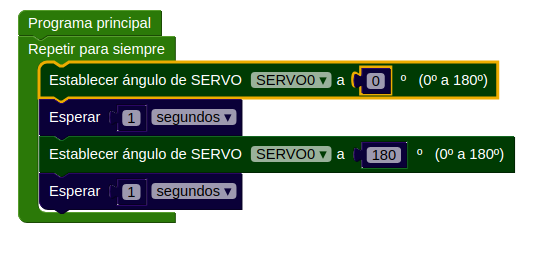
\includegraphics[width=12cm]{./Figures/debugPaso1.PNG}
		\par\caption{Resaltado del flujo de control (Parte 1).}\label{fig:debugPaso1}
	\end{center}
\end{figure}

\begin{figure}[!htbp]
	\begin{center}  % [width=10cm,height=5cm] [width=\textwidth]
		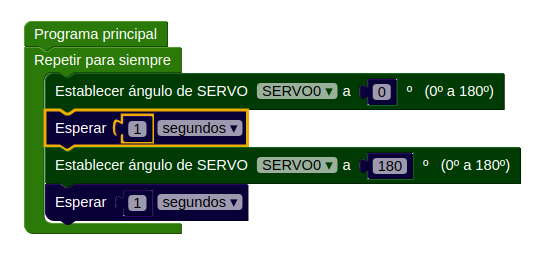
\includegraphics[width=12cm]{./Figures/debugPaso2.PNG}
		\par\caption{Resaltado del flujo de control (Parte 2).}\label{fig:debugPaso2}
	\end{center}
\end{figure}

\begin{figure}[!htbp]
	\begin{center}  % [width=10cm,height=5cm] [width=\textwidth]
		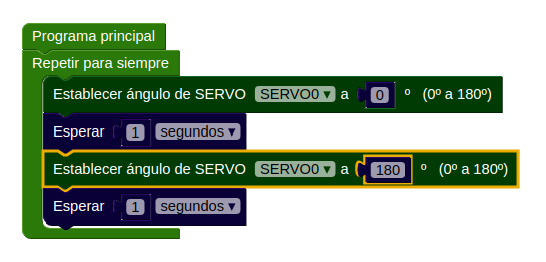
\includegraphics[width=12cm]{./Figures/debugPaso3.PNG}
		\par\caption{Resaltado del flujo de control (Parte 3).}\label{fig:debugPaso3}
	\end{center}
\end{figure}

La interfaz gráfica de usuario permite indicar al depurador cuándo pausar un programa, mediante el estableciendo de puntos de interrupción (\emph{breakpoints}).
Para establecer un de punto de interrupción, el entorno permite que el usuario haga click en el bloque en donde quiere pausar el programa. Cuando la ejecución del programa llege a este punto, el programa se detendrá. En la figura \ref{fig:add-breakpoint} se muestra el menú contextual del bloque desde donde se puede establecer el punto de interrupción.

\begin{figure}[!htbp]
	\centering
	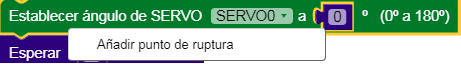
\includegraphics[width=10cm]{./Figures/add-breakpoint.PNG}
	\caption{Establecer una bandera de punto de interrupción.}
	\label{fig:add-breakpoint}
\end{figure}

Cuando se hace click en el bloque, debería mostrar un círculo rojo. Esto significa que el punto de interrupción se establece en ese bloque (figura \ref{fig:breakpoint}).

\begin{figure}[!htbp]
	\centering
	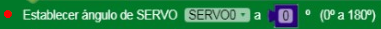
\includegraphics[width=10cm]{./Figures/breakpoint.PNG}
	\caption{Punto de interrupción.}
	\label{fig:breakpoint}
\end{figure}

Para eliminar el punto de interrupción del bloque, el usuario podrá removerlo desde el menú contextual del mismo bloque. Despues de realizar la acción, el circulo rojo del bloque se eliminará. Se ilustra el menú contextual en la figura \ref{fig:breakpoint-eliminar}.

\begin{figure}[!htbp]
	\centering
	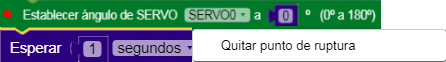
\includegraphics[width=10cm]{./Figures/breakpoint-eliminar.PNG}
	\caption{Quitar Punto de interrupción.}
	\label{fig:breakpoint-eliminar}
\end{figure}

Utilizando el botón \emph{Desactivar puntos de interrupción}, el entorno permite al alumno desactivar todos sus puntos de interrupción a la vez, sin eliminarlos, recordando cuales desactivo, entonces si se hace click nuevamente vuelven al estado original.
En la siguiente figura \ref{fig:desactivar-breakpoints} se muestra el ícono de este botón.

\begin{figure}[!htbp]
	\begin{center}  % [width=10cm,height=5cm] [width=\textwidth]
		
\includegraphics[scale=.90]{./Figures/desactivar-breakpoints.PNG}
		\par\caption{Desactivar los Puntos de interrupción activos.}\label{fig:desactivar-breakpoints}
	\end{center}
\end{figure}

\subsection{Menú de visualización}
\label{subsec:Iniciar/Menú de visualización}

El menú de visualización se divide en dos áreas, una para visualización de variables y otra para puntos de ruptura. La primera permite observar como cambian las variables de programa a medida que se ejecuta mientras está activa la sesión de depuración. En la siguiente figura \ref{fig:ventana-variables} se muestra el panel de variables.

\begin{figure}[!htbp]
	\centering
	\includegraphics*[width=9cm,height=3cm]{./Figures/variables.PNG}
	\caption{Menú de visualización de variables.}
	\par\label{fig:ventana-variables}
\end{figure}

La segunda, permite la visualización de todos los puntos de ruptura (\emph{breakpoints}) insertados en el programa, se permite modificar el estado activo/inactivo de cada punto de ruptura. En la siguiente figura \ref{fig:ventana} se muestra la ventana de \emph{breakpoints}.

\begin{figure}[!htbp]
	\centering
	\includegraphics*[width=8cm,height=2cm]{./Figures/breakpoints.PNG}
	\caption{Ventana de Puntos de ruptura (\emph{breakpoints}).}
	\par\label{fig:ventana}
\end{figure}

El entorno maneja la ejecución en los siguientes estados:

\begin{itemize}
	\item Ejecución de bloque sin breakpoint.
	\item Ejecución de bloque con breakpoints activos.	
	\item Ejecución de bloque con breakpoints inactivos.
\end{itemize}


\section{Edición de programa}
\label{sec:Edición de programa}

El área de edición de programa del entorno del \emph{debug}, contiene la misma estructura de bloques de la caja de herramientas de CIAABOT IDE, las cuales se dividen en las siguientes categorías:

\begin{itemize}
	\item Lógica.
	\item Entradas/Salidas.	
	\item Servo.
	\item Tiempo.
	\item Control.
	\item Variables.
	\item Funciones.
	\item Matemática.
	\item Texto.
\end{itemize}

El propósito, es permitir la modificación del programa cuando el usuario encuentre errores en la sesión de debug y quiera corregirlo en el entorno del \emph{debug}, de esta manera no tendrá la necesidad de guardar el programa para recién poder editarlo en CIAABOT IDE.


\section{Implementación}
\label{sec:Implementación}

\emph{CIAABOT Debug} esta desarrollado en el lenguaje Javascript. Permite importar un proyecto desde CIAABOT IDE con extensión .cbp y genera internamente código javascript para ejecutar la misma lógica que el programa en bloques. 
Para realizar esto se utiliza el archivo .cbp tiene la estructura de archivo de texto xml. Se separan los bloques gráficos que acceden a los periféricos de los bloques gráficos que no acceden a los periféricos, generando de esta manera el código correspondiente que integra todas las partes para que cuando se realice la ejecución del programa, lo haga de forma transparente para el usuario.

Mediante el cliente firmata Johnny-Five se establece la comunicación entre la aplicación y la placa EDU-CIAA-NXP, para el manejo de los periféricos. Johnny-Five es un cliente firmata, basado en el lenguaje javaScript, y dentro del entorno de \emph{debug}, es el encargado de interactuar con el microcontrolador con Firmata4CIAA para la manipulación de los periféricos.
En la siguiente figura \ref{fig:diagrama-bloques} se muestra el diágrama de bloques.

\begin{figure}[!htbp]
	\centering
	\includegraphics*[width=13cm]{./Figures/diagrama-bloques-2.PNG}
	\caption{Diágrama de Bloques para el manejo de los periféricos.}
	\par\label{fig:diagrama-bloques}
\end{figure}

\subsection{Implentación de la GUI}
\label{subsec:Implentación de la GUI}

A continuación se explicara las partes de bloques gráficos que ejecutan solo código javascript y las partes que ejecutan comandos de johnny five.

A modo de ejemplo, en la figura \ref{fig:codigo-servo-bloques} cómo se armaría en bloques el código para el barrido angular de un servomotor.

\begin{figure}[!htbp]
	\centering
	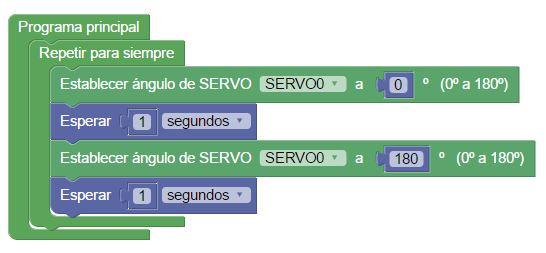
\includegraphics[width=12cm]{./Figures/ejemplo-servo.jpg}
	\caption{Ejemplo de código en bloques para el barrido de un servo.}
	\label{fig:codigo-servo-bloques}
\end{figure}

El código de salida en lenguaje Javascript de la figura \ref{fig:codigo-servo-bloques} se muestra 
en el Algoritmo 3.1:


\begin{lstlisting}[caption={Salida del código en bloques de la figura \ref{fig:codigo-servo-bloques}.}\label{cod:codigo-servo-c}] 
		                while(true){
			                	ciaa.setServo(0);
			                	wait.for(1, sec);
				                ciaa.setServo(180);
				                wait.for(1, sec);
		                };

\end{lstlisting}


\begin{itemize}
	\item Bloques gráficos que acceden a los periféricos: son aquellos que usarán el protocolo firmata para enviar comandos a la placa, y mediante las funciones por UART se van comunicando con el hardware. Por ejemplo en el manejo de sensores, motores, etc. En la figura \ref{fig:servoj5} se muestra un bloque de este tipo.
	
	
	\begin{figure}[!htbp]
		\centering
		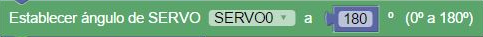
\includegraphics[width=12cm]{./Figures/ejemplo-servo-j5.PNG}
		\caption{Barrido de servomotor ejecutado con johnny five}
		\label{fig:servoj5}
	\end{figure}
   
    \begin{lstlisting}[caption={Código que ejecuta una de las funciones de johnny five del bloque de la figura \ref{fig:servoj5}.}\label{cod:codigo-servo-j5}] 
                  setServo: function(range) {
                    servo.to(range);
                  }
    \end{lstlisting}
	
	\item Bloques gráficos que no acceden a los periféricos: son aquellos que se ejecutan en la misma pc, por medio de javascript. Por ejemplo las sentencias loop-for, if-else, etc.  En la figura \ref{fig:waitj} se muestra un bloque de este tipo.
	
	\begin{figure}[!htbp]
		\centering
		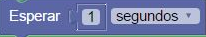
\includegraphics[width=6cm]{./Figures/ejemplo-servo-j.PNG}
		\caption{Ejemplo de wait}
		\label{fig:waitj}
	\end{figure}

	\begin{lstlisting}[caption={Código en javascript del bloque de la figura \ref{fig:waitj}.}\label{cod:codigo-servo-j}] 
			       for: function(time, unit) {
				        duration = time;
			        	waitStart = getTime(unit);
		           }
	\end{lstlisting}
\end{itemize}

En la figura \ref{fig:servoj5} se expone el bloque gráfico que utiliza los comandos de la API Johnny-five.io. A modo de ejemplo se hizo referencia a un bloque gráfico que usa la siguiente función: 

\emph{to(degrees 0-180 [, ms [, rate]])// establece la posición de 0 a 180 grados}


La figura \ref{fig:DocSecuencia} muestra el diagrama de secuencia del acceso a un periférico mediante el protocolo firmata.


\begin{figure}[!htbp]
	\begin{center}  % [width=10cm,height=5cm] [width=\textwidth]
		\includegraphics*[width=15cm]{./Figures/DocSecuencia.PNG}
		\par\caption{Diagrama de secuencia.}\label{fig:DocSecuencia}
	\end{center}
\end{figure}


\subsection{Herramientas utilizadas}
\label{subsec:Implementación del modelo computacional Servicios}

Para el desarrollo del entorno de \emph{debugger} se utilizaron los siguientes proyectos de código abierto:

\begin{itemize}
	\item Blockly \citep{blockly}: el lenguaje gráfico de CIAABOT IDE esta basado en esta biblioteca, por lo cual fue necesario la implementación de ciertas rutinas de código en javascript con la biblioteca blockly para lograr la visualización de los diagramas de bloques creados en CIABOOT IDE, así como también la manipulación de estos bloques gráficos para lograr la interacción con el interprete de Javascript. 
	
	\item Bootstrap \citep{bootstrap}: se uso esta biblioteca dentro de la aplicación para darle comportamiento a los botones del entorno del \emph{debug}, ya que provee todas las reglas CSS y HTML5 y se integra muy bien con las bibliotecas de javascript que usa el entorno.
	
	\item JS-Interpreter \citep{js-Interpreter}: el proyecto utiliza este intérprete de JavaScript ya que permite la ejecución línea por línea de código JavaScript generado para ejecutar el programas de usuario en bloques, y también para resaltar los bloques del programa a medida que se vayan ejecutando internamente. De esta manera los estudiantes podrán realizar un paso a través de su código para ver qué hace qué durante la depuración. 

	\item Acorn \citep{acorn}: es un rápido analizador tolerante a errores de JavaScript escrito en JavaScript, el analizador dentro del proyecto es usado para darle soporte al análisis/lectura de código del interprete de JavaScript.
	
	\item JQuery \citep{jQuery}: la biblioteca multiplataforma de JavaScript permite interactuar con los documentos HTML, manipular el árbol DOM de la página, agregar dinamismo a la aplicación y manejar eventos.
	
	\item Signals \citep{signals}: biblioteca escrita en JavaScript que implementa el patrón publicación/suscripción para agregar emisores de eventos al código cuando los bloques gráficos que se están ejecutando son resaltados.
	
	\item Johnny five \citep{johnny}: esta basado en Node.js y se integra muy bien con bibliotecas javascript que usamos en el entorno. Se utliza para la comunicación con la EDU-CIAA-NXP y trabajar con sus periféricos.
	
	\item Express \citep{express}: \emph{framework} de aplicación web ligero, rápido y muy útil, esta basado en http para Node.js, se usa para crear la aplicaciones web que luego son embebidas en una aplicación de escritorio. Esta biblioteca  proporciona funcionalidades como el enrutamiento, opciones para gestionar sesiones y cookies.
	
	\item Serialport \citep{serialport}: junto a firmata es usada para combinar JavaScript y hardware. Esta biblioteca permite el acceso a puertos series en la computadora.
	
	\item Electron \citep{electron}: permite armar el desarrollo de la aplicación de escritorio multiplataforma utilizando tecnologías web.
\end{itemize}


\subsection{Archivo de estado de \emph{CIAABOT Debug}}
\label{subsec:Archivo de CIAABOT Debug}

Cuando se abre un proyecto (archivo \emph{.cbp}), se crea un archivo \emph{.cbd} donde se guardan los puntos de interrupción que utiliza el usuario durante su sesión de depuración.

El archivo \emph{.cbd} se implementa mediante un archivo de texto en formato JSON \citep{json}. El mismo se guarda al cerrar el proyecto. De esta forma se recuperan los puntos de interrupción que fueron agregados al programa
y si se encuentran activos o no, de acuerdo a la elección realizada por el usuario en la última sesión de depuración. 

Si un proyecto luego es modificado por CIAABOT IDE, por ejemplo eliminando algún bloque que contenía un \emph{breakpoint}, al abrirlo nuevamente desde\emph{ CIAABOT Debug} se actualiza la información del archivo .cbd asociada al proyecto .cbp para mantener la coherencia entre los mismos.

Esta información es útil cuando el usuario cerro por algún motivo el entorno de \emph{CIAABOT Debug} y cuando lo vuelve a abrir no pierde el estado de los puntos de interrupciones utilizados en su última sesión de depuración.

En el Algoritmo 3.4 se expone un ejemplo de la estructura del archivo nombrado \emph{debug.cbd}.

\lstset{
	string=[s]{"}{"},
	stringstyle=\color{blue},
	comment=[l]{:},
	commentstyle=\color{black},
}

\begin{lstlisting}[caption={Estructura del archivo \emph{debug.cbd}} \label{cod:json}] 
{
  "type": "ciaabotDebugState",
  "breakpoins": [
     {
       "type": "asociation",
       "key": {
               "type": "logic_operation\",
               "id": "Ju6).aSXM}[dFL_Xw/p,\"
              },
       "value": {
                "type": "breakpoint",
                "id": 1,
                "active" : true
                }
     }, 
     {
       "type": "asociation",
       "key": {
               "type": "ciaa_sapi_gpio_digital_read",
               "id": "Oj7~RU|??CeufGPNV$|W\"
              },
       "value": {
                "type": "breakpoint",
                "id": 2,
                "active" : false
                }
      }
    ]
}
\end{lstlisting}


\subsection{GitLab}
\label{subsec:GitLab}

Como estrategia de mitigación del riesgo de pérdida de código, se propuso el versionado de código, para realizarlo se eligió la herramienta Gitlab, que es un servicio web de control de versiones y desarrollo de software colaborativo. Esta basado en Git y permite repositorios de código públicos y privados. 

